% Factorial staircases. Build: latexmk -pdf main.tex
% Figures: python3 make_figures.py   Tables: python3 make_tables.py
% Every identity is checked by ../verification/verify.py.
\documentclass[11pt]{amsart}

\usepackage[margin=1.15in]{geometry}
\usepackage{amsmath,amssymb,amsthm}
\usepackage{booktabs}
\usepackage{array}
\usepackage{graphicx}
\usepackage{xcolor}
\usepackage{listings}
\usepackage{embedfile}
\lstset{basicstyle=\ttfamily\footnotesize,columns=fullflexible,keepspaces=true,
  frame=single,framerule=0.3pt,rulecolor=\color{black!30},xleftmargin=6pt,
  xrightmargin=6pt,literate={≤}{{$\le$}}1 {ℕ}{{$\mathbb{N}$}}1 {∑}{{$\sum$}}1
  {∈}{{$\in$}}1 {Σ}{{$\Sigma$}}1 {·}{{$\cdot$}}1}
\usepackage[colorlinks=true,linkcolor=blue!50!black,citecolor=blue!50!black,urlcolor=blue!50!black]{hyperref}

\theoremstyle{plain}
\newtheorem{theorem}{Theorem}[section]
\newtheorem{proposition}[theorem]{Proposition}
\newtheorem{lemma}[theorem]{Lemma}
\newtheorem{corollary}[theorem]{Corollary}
\theoremstyle{definition}
\newtheorem{definition}[theorem]{Definition}
\newtheorem{example}[theorem]{Example}
\newtheorem{question}[theorem]{Question}
\theoremstyle{remark}
\newtheorem{remark}[theorem]{Remark}

\newcommand{\Sym}{\mathfrak{S}}
\newcommand{\lex}{<_{\mathrm{lex}}}
\newcommand{\lexeq}{\le_{\mathrm{lex}}}
\newcommand{\rank}{\operatorname{rank}}
\newcommand{\inv}{\operatorname{inv}}
\newcommand{\qint}[1]{[#1]_q}
\newcommand{\qfact}[1]{[#1]_q!}

\begin{document}

% Supporting files, attached to the PDF (see Appendix B).
\embedfile[filespec=verify.py]{../verification/verify.py}
\embedfile[filespec=near\string_kurepa.py]{../verification/near_kurepa.py}
\embedfile[filespec=near\string_kurepa.c]{../verification/near_kurepa.c}
\embedfile[filespec=Basic.lean]{../lean/FactorialStaircases/Basic.lean}
\embedfile[filespec=Arithmetic.lean]{../lean/FactorialStaircases/Arithmetic.lean}
\embedfile[filespec=Axioms.lean]{../lean/FactorialStaircases/Axioms.lean}
\embedfile[filespec=Lean-README.md]{../lean/README.md}

\title[Factorial staircases]{Factorial staircases:\\
a pattern in factorials, explained}
\author{Vaibhav Sanghai}
\date{\today}
\subjclass[2020]{05A05, 05A19, 11A07, 11A63, 11B65}
\keywords{factorial, lexicographic order, Lehmer code, factorial number system,
mixed radix, left factorial, Kurepa's conjecture, derangement, Wilson's theorem}

\begin{abstract}
This expository note starts from a pattern found by experiment. The expression
$(n-m)\bigl[(n-1)!+(n-2)!+\dots+(n-m-1)!\bigr]$ equals $n!$ when $m=1$ but falls
short of $n!$ when $m\ge2$, and the shortfall is always
$(m-1)(n-1)!+(m-2)(n-2)!+\dots+1\cdot(n-m+1)!$. We prove the pattern and
explain it with the factorial number system. The shortfall is the number of
permutations of $1,\dots,n$ that come before, in dictionary order, the
permutation that reverses the first $m$ entries. Changing the multiplier leads
to Kurepa's left factorial $!n=0!+1!+\dots+(n-1)!$. Modulo a prime $p$, the
bracket (with an obvious factorial removed) depends only on $n$ modulo $p$.
Its value is an alternating sum of falling factorials. When $m-n$ is
congruent modulo $p$ to some $j\le m$ (for example when $n=p$, the case
relevant to Kurepa's conjecture), this sum equals $(-1)^jd_j$, where $d_j$ is a
derangement number; otherwise it is a truncation of that sum. This is a direct extension of a
lemma of Kellner. Nothing here needs more than telescoping sums, Lehmer codes
and Wilson's theorem. The aim is to show how a simple observation leads to
these classical ideas, not to present new theorems.
\end{abstract}

\maketitle

% ===========================================================================
\section{Introduction}\label{sec:intro}
% ===========================================================================

Since $n!=n\cdot(n-1)!$ and $n=(n-1)+1$, we can write
\begin{equation}\label{eq:first}
  n!=(n-1)\bigl[(n-1)!+(n-2)!\bigr].
\end{equation}
For $n=7$ this reads $5040=6\cdot(720+120)$. A natural guess for the next
formula of this kind is to lower the multiplier by one and add one more
factorial to the bracket:
\[
  (n-2)\bigl[(n-1)!+(n-2)!+(n-3)!\bigr].
\]
This is not equal to $n!$. For $n=7$ it equals $5\cdot(720+120+24)=4320$, which
is $720$ less than $7!$. The missing amount, $720$, is exactly $6!=(n-1)!$, and
the same happens for every $n\ge3$. Continuing in the same way gives
Table~\ref{tab:staircase}. The shortfall is always a ``staircase'': a sum of
factorials whose coefficients go down by one.

\begin{table}[!ht]
\centering
\begin{tabular}{@{}cll@{}}
\toprule
$m$ & multiplier & shortfall $\;n!-(\text{multiplier})\cdot\bigl[(n-1)!+\dots+(n-m-1)!\bigr]$\\
\midrule
$1$ & $n-1$ & $0$\\
$2$ & $n-2$ & $(n-1)!$\\
$3$ & $n-3$ & $2(n-1)!+(n-2)!$\\
$4$ & $n-4$ & $3(n-1)!+2(n-2)!+(n-3)!$\\
$5$ & $n-5$ & $4(n-1)!+3(n-2)!+2(n-3)!+(n-4)!$\\
\bottomrule
\end{tabular}
\caption{The shortfall for the first five values of $m$. The bracket contains
$m+1$ factorials.}
\label{tab:staircase}
\end{table}

\subsection*{Notation}
For integers $0\le m\le n-1$ we write
\[
  L_m(n)=\sum_{i=1}^{m+1}(n-i)!=(n-1)!+(n-2)!+\dots+(n-m-1)!
\]
for the bracket, and
\[
  R_m(n)=n!-(n-m)\,L_m(n)
\]
for the shortfall. The table suggests
$R_m(n)=\sum_{i=1}^{m-1}(m-i)(n-i)!$.

\subsection*{Outline}
Section~\ref{sec:identity} proves this formula for all $m$ and $n$
(Proposition~\ref{thm:identity}). The proof is short, but it does not explain why
the multiplier must be $n-m$, so the same section gives a second proof that
does (Proposition~\ref{thm:lex}). List all permutations of
$1,2,\dots,n$ in dictionary order. Then $R_m(n)$ is the number of permutations
that come before the permutation
\[
  w_m=m\,(m-1)\cdots2\,1\,(m+1)\,(m+2)\cdots n,
\]
which reverses the first $m$ entries. The multiplier $n-m$ is the number of
ways to move past $w_m$ at each of its first $m$ positions.

The rest of the note follows one thread, from this identity to a classical
open problem. Each result is a short consequence of Lemma~\ref{lem:rank}, of
the telescoping argument in Proposition~\ref{thm:identity}, or of Kellner's
lemma; we include them as illustrations of these tools, not as new theorems.
\begin{itemize}
  \item Section~\ref{sec:family}: any multiplier $c$ with $1\le c\le n-m$ gives
        a similar identity, attached to a different permutation. Taking $m=n-1$
        brings in Kurepa's left factorial $!n=0!+1!+\dots+(n-1)!$.
  \item Section~\ref{sec:arith}: modulo a prime $p$, the bracket $L_m(n)$,
        after dividing out $(n-m-1)!$, depends only on $n$ modulo $p$. Its
        value is a truncated alternating sum of falling factorials
        (Proposition~\ref{thm:period}). Let $j$ be the residue of $m-n$
        modulo~$p$. If $j\le m$, which always holds when $n=p$, this sum is
        $(-1)^jd_j$, where $d_j$ is a derangement number. If $j>m$ it is a
        truncation of that sum. The case $n=p$ is a lemma of Kellner,
        which restates Kurepa's conjecture.
\end{itemize}
Section~\ref{sec:open} lists questions for further study.
Appendix~\ref{app:var} collects side variations that use the same tools (other
products such as double factorials, and a $q$-analogue). Appendix~\ref{app:data} describes the computer checks
and the formal proofs.

\subsection*{What is known}
All results in this note are elementary, and most are standard or close to
standard.
\begin{itemize}
  \item Proposition~\ref{thm:identity} is a rearrangement of the classical
        telescoping identity $\sum_{j=0}^{n-1}j\cdot j!=n!-1$ \cite{GKP}.
  \item Lemma~\ref{lem:rank} is the factorial number system of
        Laisant~\cite{Laisant} and Lehmer~\cite{Lehmer}; see also
        \cite[\S7.2.1.2]{TAOCP4A}. Propositions~\ref{thm:lex}
        and~\ref{thm:family} are direct applications of it, and
        Proposition~\ref{thm:mixed} is the same argument for a mixed-radix
        number system~\cite{TAOCP2,Fraenkel}.
  \item The numbers $R_m(n)$ already appear in the OEIS in two special cases.
        For $m=3$, $R_3(n)$ is term $n-2$ of A052649~\cite{A052649} (offset
        $0$), where a 2004 comment by Eugene McDonnell notes the
        interpretation with three reversed entries. For $m=n-1$,
        $R_{n-1}(n)=n!-{!n}$ is term $n$ of A065355~\cite{A065355}.
  \item Proposition~\ref{thm:q} is the usual refinement of a counting argument
        by inversions~\cite[Ch.~1]{EC1}.
  \item Proposition~\ref{thm:period} is a short extension of
        \cite[Lemma~2.4]{Kellner}, which is the case $n=p$. Kellner restates
        Kurepa's conjecture~\cite{Kurepa,Guy} as $p\nmid d_{p-1}$ in
        \cite[Lemma~2.1 and Corollary~2.2]{Kellner}; see also
        Me\v{s}trovi\'c~\cite{Mestrovic} and, for recent equivalent forms of
        the conjecture, Petojevi\'c et al.~\cite{Petojevic2023}.
  \item The primes in Table~\ref{tab:nearkurepa} can be read off from the
        residues of $!p$ modulo $p$, which are tabulated in OEIS
        A100612~\cite{A100612}. Its row $k=2$ is A258944~\cite{A258944}.
\end{itemize}
We have not seen the general statements written down in exactly this form,
but specialists would regard them as routine. For this reason we call them
propositions rather than theorems. Every result was checked by computer, and
most were also proved formally in the proof assistant Lean~4 with the Mathlib
library. Appendix~\ref{app:data} lists what was checked and how. The scripts
and Lean files are at
\url{https://github.com/VaibhavSanghai13/factorial-staircases} and are also
attached to this PDF.

% ===========================================================================
\section{Permutations in dictionary order}\label{sec:prelim}
% ===========================================================================

Let $\Sym_n$ be the set of permutations of $\{1,\dots,n\}$, written as words
$w=w_1w_2\cdots w_n$. We compare two permutations the way a dictionary compares
words. Look at the first position where they differ; the one with the smaller
entry there comes first. We write $u\lex w$ when $u$ comes before $w$. The
\emph{rank} of $w$ is the number of permutations that come before it:
\[
  \rank(w)=\#\{u\in\Sym_n : u\lex w\}.
\]
The first permutation $12\cdots n$ has rank $0$, and the last one,
$n\cdots21$, has rank $n!-1$.

There is a simple formula for the rank. For each position $i$, let
\[
  \ell_i(w)=\#\{j>i : w_j<w_i\},\qquad g_i(w)=\#\{j>i : w_j>w_i\}.
\]
These count the entries to the right of position $i$ that are smaller and
larger than $w_i$. Since there are $n-i$ entries to the right of position $i$,
we have $\ell_i(w)+g_i(w)=n-i$. The list $\ell_1(w),\dots,\ell_n(w)$ is called
the \emph{Lehmer code} of $w$ \cite{Lehmer,Laisant}.

\begin{lemma}[factorial number system \cite{Lehmer,TAOCP4A}]\label{lem:rank}
For every $w\in\Sym_n$,
\[
  \rank(w)=\sum_{i=1}^{n}\ell_i(w)\,(n-i)!
  \qquad\text{and}\qquad
  \#\{u\in\Sym_n : w\lexeq u\}=1+\sum_{i=1}^{n}g_i(w)\,(n-i)!.
\]
\end{lemma}

\begin{proof}
Take $u\neq w$, and let $i$ be the first position where they differ. The
entries still unused at position $i$ are exactly $w_i,w_{i+1},\dots,w_n$. If
$u_i$ is one of the $\ell_i(w)$ entries smaller than $w_i$, then $u$ comes
before $w$. If it is one of the $g_i(w)$ entries larger than $w_i$, then $u$
comes after $w$. In either case the remaining $n-i$ positions can be filled in
$(n-i)!$ ways. Summing over $i$ gives both formulas; the extra $1$ in the
second formula counts $w$ itself.
\end{proof}

\begin{example}
For $w=3214$: the entry $3$ has two smaller entries to its right, so
$\ell_1=2$. The entry $2$ has one, so $\ell_2=1$. Hence
$\rank(3214)=2\cdot3!+1\cdot2!=14$. Indeed, $3214$ is the fifteenth
permutation of $\{1,2,3,4\}$ in dictionary order.
\end{example}

% ===========================================================================
\section{The staircase identity and what it counts}\label{sec:identity}
% ===========================================================================

\begin{proposition}[staircase identity; a form of $\sum j\cdot j!=n!-1$]\label{thm:identity}
For all integers $0\le m\le n-1$,
\[
  n!=(n-m)\sum_{i=1}^{m+1}(n-i)!\;+\;\sum_{i=1}^{m-1}(m-i)\,(n-i)!.
\]
In other words, $R_m(n)=\sum_{i=1}^{m-1}(m-i)(n-i)!$.
\end{proposition}

\begin{proof}
The only fact we need is $j\cdot j!=(j+1)!-j!$. Write the multiplier as
$n-m=(n-i)-(m-i)$, and treat the two parts separately. First,
\[
  \sum_{i=1}^{m+1}(n-i)\,(n-i)!=\sum_{i=1}^{m+1}\bigl[(n-i+1)!-(n-i)!\bigr]
  =n!-(n-m-1)!,
\]
because the sum telescopes. Second, in $\sum_{i=1}^{m+1}(m-i)(n-i)!$ the term
$i=m$ is zero and the term $i=m+1$ is $-(n-m-1)!$, so
\[
  \sum_{i=1}^{m+1}(m-i)\,(n-i)!=\sum_{i=1}^{m-1}(m-i)\,(n-i)!-(n-m-1)!.
\]
Subtracting the second equation from the first gives
$(n-m)L_m(n)=n!-\sum_{i=1}^{m-1}(m-i)(n-i)!$.
\end{proof}

\begin{remark}\label{prop:gamma}
The proof uses only $j\cdot j!=(j+1)!-j!$, so it also works for the Gamma
function, which satisfies $\Gamma(z+1)=z\,\Gamma(z)$. For an integer $m\ge0$
and a complex number $x$ that is not one of $m,m-1,m-2,\dots$,
\[
  \Gamma(x+1)=(x-m)\sum_{i=1}^{m+1}\Gamma(x-i+1)+\sum_{i=1}^{m-1}(m-i)\,\Gamma(x-i+1),
\]
by the same telescoping with $(x-i)\Gamma(x-i+1)=\Gamma(x-i+2)-\Gamma(x-i+1)$.
\end{remark}

The proof works, but it does not explain where the multiplier $n-m$ comes
from. The next proposition does.

\begin{proposition}[for $m=3$, see \cite{A052649}]\label{thm:lex}
Let $0\le m\le n-1$ and $w_m=m\,(m-1)\cdots1\,(m+1)\cdots n$. Then
\[
  \rank(w_m)=\sum_{i=1}^{m-1}(m-i)(n-i)!=R_m(n)
  \quad\text{and}\quad
  \#\{u\in\Sym_n: w_m\lexeq u\}=(n-m)\sum_{i=1}^{m+1}(n-i)!.
\]
So Proposition~\ref{thm:identity} says that the permutations before $w_m$ and the
permutations from $w_m$ on together make up all $n!$ permutations.
\end{proposition}

\begin{proof}
For $i\le m$ the entry of $w_m$ in position $i$ is $m-i+1$. All the smaller
values $1,\dots,m-i$ lie to its right, and so do all the $n-m$ values
$m+1,\dots,n$, which are larger. After position $m$ the entries increase. So
\[
  \ell_i(w_m)=m-i,\quad g_i(w_m)=n-m\qquad(i\le m),
\]
\[
  \ell_i(w_m)=0,\quad g_i(w_m)=n-i\qquad(i>m).
\]
By Lemma~\ref{lem:rank}, $\rank(w_m)=\sum_{i=1}^{m}(m-i)(n-i)!$, and the term
$i=m$ is zero. For the second count, Lemma~\ref{lem:rank} gives
\[
  (n-m)\sum_{i=1}^{m}(n-i)!+\Bigl(1+\sum_{i=m+1}^{n}(n-i)(n-i)!\Bigr)
  =(n-m)\sum_{i=1}^{m}(n-i)!+(n-m)!,
\]
and $(n-m)!=(n-m)\,(n-m-1)!$ supplies the last term of the bracket.
\end{proof}

The proof shows the meaning of each part of the identity. Build a permutation
from left to right, comparing it with $w_m$. At each of the first $m$
positions, the available values split into smaller ones, which put the
permutation before $w_m$, and larger ones, which put it after. There are
$m-i$ smaller values at position $i$, and their contributions form the
staircase. There are always exactly $n-m$ larger values, namely $m+1,\dots,n$,
and this constant is the multiplier. Figures~\ref{fig:tree}
and~\ref{fig:choices} show this.

\begin{figure}[!ht]
\centering
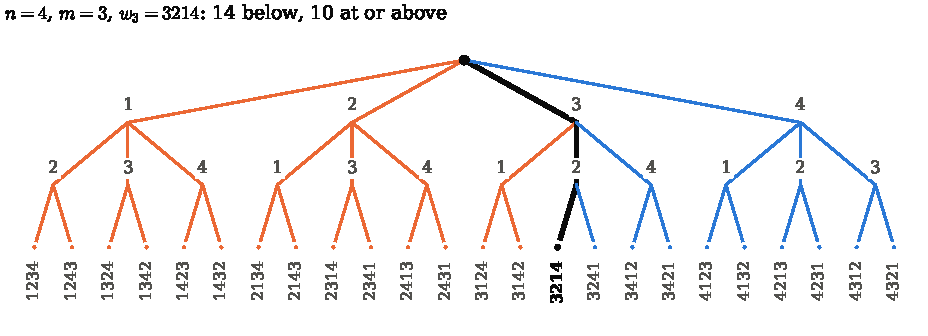
\includegraphics[width=\linewidth]{figures/lex_tree.pdf}
\caption{The $24$ permutations of $\{1,2,3,4\}$ as a tree, read from top to
bottom; the leaves are in dictionary order. The black path leads to
$w_3=3214$. Orange: the $R_3(4)=14$ permutations before it. Blue: $3214$ and
the $9$ permutations after it. At each of the first three levels, the black
path has exactly $n-m=1$ blue branch to its right.}
\label{fig:tree}
\end{figure}

\begin{figure}[!ht]
\centering
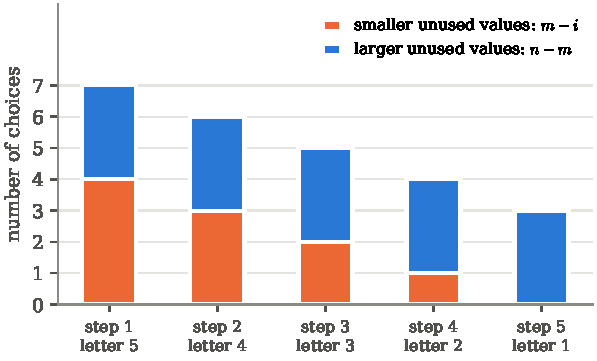
\includegraphics[width=0.66\linewidth]{figures/choices.pdf}
\caption{The choices at each of the first five positions of
$w_5=54321678\in\Sym_8$. Orange: values smaller than the entry of $w_5$
($4,3,2,1,0$). Blue: larger values (always $n-m=3$).}
\label{fig:choices}
\end{figure}

\begin{example}
For $n=4$ and $m=3$ we have $w_3=3214$. Proposition~\ref{thm:lex} says that
$R_3(4)=2\cdot3!+1\cdot2!=14$ permutations come before $3214$, and
$(4-3)(3!+2!+1!+0!)=10$ permutations come from $3214$ on; $14+10=24=4!$.
\end{example}

% ===========================================================================
\section{Other multipliers}\label{sec:family}
% ===========================================================================

If we use a multiplier $c$ smaller than $n-m$, we still get an identity, but
it is attached to a different permutation.

\begin{proposition}\label{thm:family}
Let $0\le m\le n-1$ and $1\le c\le n-m$. Then
\[
  n!=c\sum_{i=1}^{m+1}(n-i)!\;+\;\sum_{i=1}^{m}(n-i-c)(n-i)!\;+\;(n-m-c)(n-m-1)!,
\]
and the last two terms together are the rank of the permutation
\[
  w_{m,c}=(n-c)\,(n-c-1)\cdots(n-c-m+1)\;\;(n-c+1)\;\;
  1\,2\cdots(n-c-m)\;\;(n-c+2)\cdots n .
\]
\end{proposition}

\begin{proof}
The word $w_{m,c}$ consists of four blocks: a decreasing block of $m$ values,
then the value $n-c+1$, then the values below the first block in increasing
order, then the values above $n-c+1$ in increasing order. The conditions
$1\le c\le n-m$ make sure these are the values $1,\dots,n$, each used once.

Each of the first $m$ entries has all smaller values to its right, since every
entry to its left is larger. So $\ell_i=n-c-i$ for $i\le m$. The entry
$n-c+1$ in position $m+1$ has $1,\dots,n-c-m$ to its right, so
$\ell_{m+1}=n-m-c$. All later entries have $\ell_i=0$. Lemma~\ref{lem:rank}
gives the rank. The identity itself follows from
\[
  \sum_{i=1}^{m}(n-i)(n-i)!+(n-m)(n-m-1)!=\bigl(n!-(n-m)!\bigr)+(n-m)!=n!
\]
by splitting $n-i=c+(n-i-c)$ and $n-m=c+(n-m-c)$.
\end{proof}

For $c=n-m$ the last term vanishes, $w_{m,c}=w_m$, and we recover
Proposition~\ref{thm:identity}. This is the only value of $c$ for which the term
with $(n-m-1)!$ disappears. That is why the pattern in
Table~\ref{tab:staircase} looks so simple.

\begin{example}
Take $n=5$, $m=2$, $c=1$. Then $w_{2,1}=43\,5\,12$, and the proposition says
$120=1\cdot(4!+3!+2!)+(3\cdot4!+2\cdot3!)+2\cdot2!=32+84+4$.
\end{example}

\begin{corollary}\label{cor:kurepa}
Let $!n=0!+1!+\dots+(n-1)!$ be Kurepa's left factorial \cite{Kurepa,A003422}.
Then
\[
  n!=\;!n+\sum_{j=1}^{n-1}(j-1)\,j!,
\]
and $!n$ is the number of permutations from $(n-1)(n-2)\cdots1\,n$ onwards.
\end{corollary}

\begin{proof}
Take $m=n-1$. Then $1\le c\le n-m$ forces $c=1$, and the bracket becomes
$\sum_{i=1}^{n}(n-i)!={!n}$.
\end{proof}

% ===========================================================================
\section{The bracket modulo a prime}\label{sec:arith}
% ===========================================================================

At the end of the family is Kurepa's left factorial $!n=L_{n-1}(n)$. Kurepa
conjectured that $!p$ is not divisible by $p$ for any odd prime
$p$~\cite{Kurepa} (see also \cite[B44]{Guy}). The conjecture is still open:
computer searches have found no counterexample with $p<2^{40}$~\cite{ABT2021},
and recent papers continue to study equivalent forms of it~\cite{Petojevic2023}.
This suggests
asking, for every $m$ and $n$, what $L_m(n)$ is modulo a prime. This section
answers that question for every prime.

\subsection{Removing the obvious factor}
Every term of $L_m(n)=(n-1)!+\dots+(n-m-1)!$ is a multiple of the smallest
one, $(n-m-1)!$. Dividing it out,
\begin{equation}\label{eq:cofactor}
  L_m(n)=(n-m-1)!\;P_m(n),
\end{equation}
where, with $a=n-m$,
\[
  P_m(n)=1+a+a(a+1)+\dots+a(a+1)\cdots(a+m-1).
\]
For example, $P_2(n)=1+(n-2)+(n-2)(n-1)=(n-1)^2$. We write
$a^{\overline{k}}=a(a+1)\cdots(a+k-1)$ and
$j^{\underline{k}}=j(j-1)\cdots(j-k+1)$, both equal to $1$ for $k=0$, so that
$P_m(n)=\sum_{k=0}^{m}a^{\overline{k}}$.

In the case that matters for Kurepa's conjecture, the answer involves the
\emph{derangement numbers} $d_j$
\cite[\S2.2]{EC1}, \cite{A000166}. These count the permutations of $j$ objects
in which no object stays in its place:
\[
  d_j=j!\sum_{i=0}^{j}\frac{(-1)^i}{i!},\qquad (d_0,d_1,d_2,\dots,d_6)=(1,0,1,2,9,44,265).
\]

\subsection{\texorpdfstring{Periodicity modulo $p$}{Periodicity modulo p}}
Modulo $p$, a product of consecutive numbers starting at $a$ looks like a
product of consecutive numbers counting down from $j$, where $j$ is the
remainder of $-a$.

\begin{lemma}\label{lem:rising}
Let $p$ be prime, and let $a\equiv-j\pmod p$ with $0\le j\le p-1$. Then
$a^{\overline{k}}\equiv(-1)^k j^{\underline{k}}\pmod p$ for all $k\ge0$. In
particular $a^{\overline{k}}\equiv0$ when $k>j$.
\end{lemma}

\begin{proof}
Each factor satisfies $a+t\equiv-(j-t)\pmod p$. If $k>j$, the factor with
$t=j$ is divisible by $p$.
\end{proof}

\begin{proposition}[extends \cite{Kellner}]\label{thm:period}
Let $p$ be prime and $0\le m\le n-1$. Let $j$ be the number in
$\{0,1,\dots,p-1\}$ with $j\equiv m-n\pmod p$. Then
\[
  P_m(n)\equiv\sum_{k=0}^{\min(m,j)}(-1)^k\,j^{\underline{k}}\pmod p .
\]
If $j\le m$, this is $(-1)^j\,d_j$. In particular, for fixed $m$ the residue
of $P_m(n)$ modulo $p$ depends only on $n$ modulo $p$.
\end{proposition}

\begin{proof}
Apply Lemma~\ref{lem:rising} to each term of $P_m(n)=\sum_{k=0}^{m}a^{\overline{k}}$
with $a=n-m\equiv-j$. The terms with $k>j$ vanish. If $j\le m$, the sum runs
over $0\le k\le j$, and substituting $i=j-k$ gives
\[
  \sum_{k=0}^{j}(-1)^k\frac{j!}{(j-k)!}=(-1)^j\,j!\sum_{i=0}^{j}\frac{(-1)^i}{i!}=(-1)^j d_j.\qedhere
\]
\end{proof}

\begin{example}
Take $m=2$, so $P_2(n)=(n-1)^2$ and $j\equiv2-n$. The proposition predicts
$P_2(n)\equiv1$ when $n\equiv2$ ($j=0$, $d_0=1$), $\equiv0$ when $n\equiv1$
($j=1$, $d_1=0$), and $\equiv1$ when $n\equiv0$ ($j=2$, $d_2=1$). Indeed
$(n-1)^2$ is $1$, $0$ and $1$ modulo $p$ in these three cases.
\end{example}

\begin{figure}[!ht]
\centering
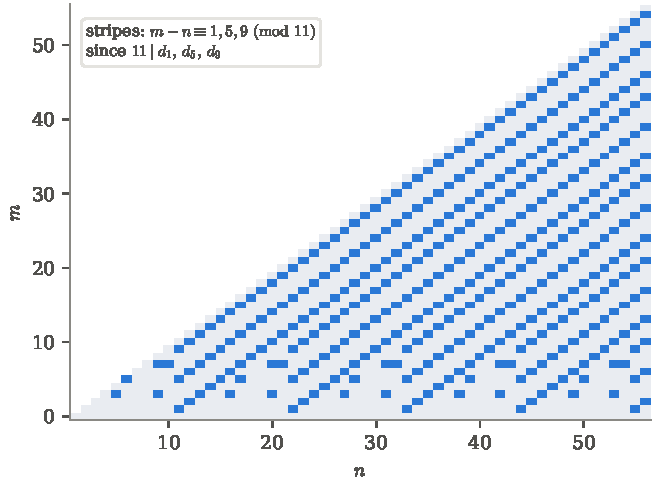
\includegraphics[width=0.6\linewidth]{figures/periodicity.pdf}
\caption{The pairs $(n,m)$ for which $11$ divides $P_m(n)$ (blue). By
Proposition~\ref{thm:period} they lie on the diagonals $m-n\equiv1,5,9\pmod{11}$,
because $11$ divides $d_1=0$, $d_5=44$ and $d_9=133496$. Near the bottom edge,
where $j>m$, the shortened sum applies instead.}
\label{fig:period}
\end{figure}

\subsection{\texorpdfstring{The case $n=p$: Kellner's lemma and Kurepa's conjecture}{The case n=p: Kellner's lemma and Kurepa's conjecture}}

\begin{corollary}[{\cite[Lemma~2.4 and Lemma~2.1]{Kellner}}]\label{cor:kellner}
Let $p$ be prime and $0\le m\le p-1$. Then
\[
  (p-1)!+(p-2)!+\dots+(p-m-1)!\;\equiv\;-\frac{d_m}{m!}\pmod p .
\]
In particular $!p\equiv d_{p-1}\pmod p$, so Kurepa's conjecture is equivalent
to the statement that $p$ does not divide $d_{p-1}$ for any odd prime $p$.
\end{corollary}

\begin{proof}
For $n=p$ we have $j=m$, so $P_m(p)\equiv(-1)^m d_m$ by
Proposition~\ref{thm:period}. Wilson's theorem says $(p-1)!\equiv-1$. Since
$(p-1)!=(p-m-1)!\,(p-m)\cdots(p-1)\equiv(p-m-1)!\,(-1)^m m!$, we get
$(p-m-1)!\equiv(-1)^{m+1}/m!$, and multiplying gives the first claim. For
$m=p-1$ the right side is $-d_{p-1}/(p-1)!\equiv d_{p-1}$.
\end{proof}

\begin{example}
For $p=11$ and $m=5$, $d_5=44$ is divisible by $11$, so
$10!+9!+8!+7!+6!+5!$ is divisible by $11$.
\end{example}

Kellner states the first claim as $K(p)-K(p-l)\equiv-S(l-1)/(l-1)!$
\cite[Lemma~2.4]{Kellner}, where $K$ is the left factorial and $S$ the
derangement number; the second is his Lemma~2.1 for $n=p$.
Proposition~\ref{thm:period} shows that this congruence is one value of a
periodic pattern that holds for all $n$. For example, taking $m=n-1\ge p-1$
gives $j=p-1$, and hence $!n\equiv d_{p-1}\pmod p$ for every $n\ge p$.
Kellner does not state this directly, but it follows from his Lemma~2.1
together with his Theorem~3.3, which says that $!n$ modulo $p$ is constant for
$n\ge p$.

\subsection{\texorpdfstring{Common factors with $n!$}{Common factors with n!}}
Kurepa's conjecture is often stated as $\gcd(!n,n!)=2$ for $n\ge2$. The next
corollary describes $\gcd\bigl(L_m(n),n!\bigr)$ for every $m$.

\begin{corollary}\label{cor:gcd}
Let $0\le m\le n-1$ and $G_m(n)=\gcd\bigl(L_m(n),n!\bigr)/(n-m-1)!$. Then
\[
  G_m(n)=\gcd\bigl(P_m(n),\ (n-m)(n-m+1)\cdots n\bigr).
\]
A prime $p$ divides $G_m(n)$ if and only if both of the following hold:
\begin{enumerate}
  \item some multiple of $p$ lies among $n-m,\dots,n$;
  \item the sum in Proposition~\ref{thm:period} is divisible by $p$ (when $j\le m$,
        this means $p\mid d_j$).
\end{enumerate}
Moreover, $n-m+1$ always divides $G_m(n)$ when $m\ge1$.
\end{corollary}

\begin{proof}
Both $L_m(n)=(n-m-1)!\,P_m(n)$ and $n!=(n-m-1)!\,(n-m)\cdots n$ contain the
factor $(n-m-1)!$, which gives the formula for $G_m(n)$. A prime divides the
product $(n-m)\cdots n$ exactly when (1) holds, and divides $P_m(n)$ exactly
when (2) holds, by Proposition~\ref{thm:period}. For the last claim, the two
smallest terms of $L_m(n)$ add up to $(n-m)!+(n-m-1)!=(n-m-1)!\,(n-m+1)$, and
every other term is a multiple of $(n-m+1)!$. So $n-m+1$ divides $P_m(n)$, and
it is one of the numbers $n-m,\dots,n$.
\end{proof}

For $m=n-1$ this says $G_{n-1}(n)=\gcd(!n,n!)$ is divisible by $2$, and
Kurepa's conjecture is that it equals $2$. More generally, we may ask when
$G_m(n)$ is as small as possible, namely equal to $n-m+1$. This happens for
$862$ of the $1710$ pairs with $3\le n<60$ and $1\le m\le n-1$; the corollary
names the primes responsible in the other cases.

\subsection{Near-Kurepa primes}
Taking $m=p-1-k$ in Corollary~\ref{cor:kellner} and simplifying with Wilson's
theorem gives
\[
  !p-{!k}\;\equiv\;(-1)^k\,k!\,d_{p-1-k}\pmod p\qquad(0\le k<p).
\]
So a prime $p>k$ divides $!p-{!k}$ exactly when it divides $d_{p-1-k}$. The
case $k=0$ with $p$ odd is Kurepa's question ($p=2$ divides $!2=2$ trivially),
for which no example exists with
$p<2^{40}$~\cite{AndrejicTatarevic,ABT2021}. For $k\ge1$, examples
exist (Table~\ref{tab:nearkurepa}).

\begin{table}[!ht]
\centering
\begin{tabular}{@{}rrl@{}}
\toprule
$k$ & $!k$ & odd primes $p<2\cdot10^6$ with $p>k$ and $p\mid{!p}-{!k}$\\
\midrule
$0$ & $0$ & none\\
$1$ & $1$ & $3,\ 11$\\
$2$ & $2$ & $31,\ 373$\\
$3$ & $4$ & $5,\ 41,\ 163$\\
$4$ & $10$ & $13,\ 151$\\
$5$ & $34$ & $7,\ 11$\\
$6$ & $154$ & $283,\ 1867,\ 4099$\\
$7$ & $874$ & $103,\ 2423,\ 254039,\ 304099$\\
$8$ & $5914$ & $42961,\ 1528781$\\
\bottomrule
\end{tabular}
\caption{Odd primes dividing $!p-{!k}$, equivalently $d_{p-1-k}$. The prime
$p=2$ is left out; it divides $!2-{!0}=2$ and no other entry. The row $k=2$
is OEIS A258944~\cite{A258944}, whose next term $6855730873$ was found by
Andreji\'c and Tatarevi\'c~\cite{AndrejicTatarevic}.}
\label{tab:nearkurepa}
\end{table}

The two primes in the row $k=2$ multiply to $31\cdot373=11563$.
Me\v{s}trovi\'c~\cite{Mestrovic} showed that $11563$ is a counterexample to his
``strong Kurepa hypothesis'' about a related determinant. His criterion for an
odd composite $n$ is $d_{n-1}\equiv2\pmod n$. For each prime $p$ dividing $n$
he shows $d_{n-1}\equiv d_{p-1}\pmod p$, so for $n=31\cdot373$ the criterion
becomes $p\mid d_{p-1}-2$ for $p=31,373$; by the formula above this is
$p\mid{!p}-{!2}$. We checked directly that $d_{11562}\equiv2\pmod{11563}$.

% ===========================================================================
\section{Questions for further study}\label{sec:open}
% ===========================================================================

\begin{question}
Are there similar identities for other orders on $\Sym_n$, for example
colexicographic order, or for reversing the \emph{last} $m$ entries?
\end{question}

\begin{question}
Corollary~\ref{cor:gcd} says which primes divide $G_m(n)$, but not to which
power. What is the exact power of $p$ dividing $P_m(n)$? What proportion of
pairs $(m,n)$ have $G_m(n)=n-m+1$ as $n$ grows?
\end{question}

\begin{question}
For each fixed $k\ge1$, are there infinitely many primes $p$ with
$p\mid{!p}-{!k}$? If the residues $d_{p-1-k}\bmod p$ behaved like random
numbers, the number of such primes up to $x$ would grow like $\log\log x$.
That is slowly, but without bound, consistent with
Table~\ref{tab:nearkurepa}.
\end{question}

\begin{question}
Is there a version of Proposition~\ref{thm:q} for the major index instead of
inversions? A computation shows that the two statistics are \emph{not}
equally distributed on $\{u: w_m\lexeq u\}$ when $2\le m\le n-1$ and $n\le7$,
so such a version would have a different form.
\end{question}

\begin{question}
Does Proposition~\ref{thm:family} have a mixed-radix version, and for which
multipliers is the remainder again an equally spaced staircase?
\end{question}

% ===========================================================================
\section*{Acknowledgements}
% ===========================================================================

This work began in September 2024 as an independent project of the author, a
high-school student, with the observation recorded in
Table~\ref{tab:staircase}. An AI assistant (Claude, Anthropic) proposed the
general proofs, the interpretation in Section~\ref{sec:identity}, the
generalizations in Sections~\ref{sec:family}--\ref{sec:arith} and
Appendix~\ref{app:var}, the literature
search, the verification code and the figures.
% TODO (author): rewrite this paragraph in your own words before any submission;
% see submission/AI_CONTRIBUTION_FACTS.md.

\appendix
% ===========================================================================
\section{Variations on the identity}\label{app:var}
% ===========================================================================

This appendix collects two variations that use the same two tools, the
telescoping sum and the ranking lemma. None of them is needed for the main
text.

\subsection{Other products}\label{sec:mixed}
The proof of Proposition~\ref{thm:identity} used only one property of $n!$: it
is obtained from $(n-1)!$ by multiplying by a number. Let $r_1,r_2,\dots$ be
positive integers (the \emph{growth factors}), and put $a_0=1$ and
$a_k=r_1r_2\cdots r_k$. Factorials are the case $r_k=k$, double factorials
$2\cdot4\cdots(2k)$ the case $r_k=2k$, and powers $b^k$ the case $r_k=b$.

Permutations are replaced by digit strings. Let $W_n$ be the set of strings
$d_1d_2\cdots d_n$ with $0\le d_i\le r_{n-i+1}-1$, in dictionary order. These
are the numerals of a mixed-radix number system, where each digit has its own
base \cite[\S4.1]{TAOCP2}, \cite{Fraenkel}; for $r_k=k$ the Lehmer code turns
permutations into exactly these strings, in the same order.

\begin{proposition}\label{thm:mixed}
For $0\le m\le n-1$,
\begin{equation}\label{eq:mixed}
  a_n=r_{n-m}\sum_{i=1}^{m+1}a_{n-i}\;+\;
  \sum_{i=1}^{m}\bigl(r_{n-i+1}-r_{n-m}-1\bigr)\,a_{n-i}.
\end{equation}
If $r_k>r_{n-m}$ for $n-m<k\le n$, all coefficients are nonnegative. Then the
second sum is the number of strings before $t=t_1\cdots t_m0\cdots0$, where
$t_i=r_{n-i+1}-r_{n-m}-1$, and the first term is the number of strings from
$t$ on.
\end{proposition}

\begin{proof}
Since $a_k-a_{k-1}=(r_k-1)a_{k-1}$, the sum
$\sum_{i=1}^{m}(r_{n-i+1}-1)a_{n-i}$ telescopes to $a_n-a_{n-m}$, and
$a_{n-m}=r_{n-m}a_{n-m-1}$. Splitting
$r_{n-i+1}-1=r_{n-m}+(r_{n-i+1}-r_{n-m}-1)$ gives \eqref{eq:mixed}. For the
count, argue as in Lemma~\ref{lem:rank}: a string that first differs from $t$
at position $i\le m$ has $t_i$ smaller and $r_{n-m}$ larger choices there, and
$a_{n-i}$ ways to fill the rest.
\end{proof}

\begin{remark}\label{cor:affine}
The staircase coefficient of $a_{n-i}$ is $r_{n-i+1}-r_{n-m}-1$, so the
staircase goes down in equal steps exactly when the growth factors go up in
equal steps. For $r_k=\alpha k+\beta$ the coefficients are
$\alpha(m-i+1)-1$, independent of $n$ (Table~\ref{tab:mixed}).
\end{remark}

\begin{table}[!ht]
\centering
\begin{tabular}{@{}llll@{}}
\toprule
$a_n$ & $r_k$ & multiplier & staircase coefficients\\
\midrule
$n!$ & $k$ & $n-m$ & $m-1,\ m-2,\ \dots,\ 1,\ 0$\\
$(2n)!!=2\cdot4\cdots(2n)$ & $2k$ & $2(n-m)$ & $2m-1,\ 2m-3,\ \dots,\ 3,\ 1$\\
$(2n-1)!!=1\cdot3\cdots(2n-1)$ & $2k-1$ & $2(n-m)-1$ & $2m-1,\ 2m-3,\ \dots,\ 3,\ 1$\\
$1\cdot4\cdot7\cdots(3n-2)$ & $3k-2$ & $3(n-m)-2$ & $3m-1,\ 3m-4,\ \dots,\ 5,\ 2$\\
$b^n$ & $b$ & $b$ & $-1,\ -1,\ \dots,\ -1$\\
\bottomrule
\end{tabular}
\caption{Proposition~\ref{thm:mixed} for some sequences. For powers $b^n$ the
growth factor does not increase, the coefficients are negative, and the
identity reduces to the sum of a geometric series.}
\label{tab:mixed}
\end{table}

\subsection{\texorpdfstring{A $q$-analogue}{A q-analogue}}
An \emph{inversion} of $u$ is a pair of positions $i<j$ with $u_i>u_j$; let
$\inv(u)$ be their number. With $\qint{k}=1+q+\dots+q^{k-1}$ (and
$\qint{0}=0$) and $\qfact{k}=\qint{1}\qint{2}\cdots\qint{k}$, it is classical
that $\sum_{u\in\Sym_k}q^{\inv(u)}=\qfact{k}$ \cite[Cor.~1.3.13]{EC1}.

\begin{proposition}[cf.\ \cite{EC1}]\label{thm:q}
For $0\le m\le n-1$ let $e_i=\sum_{j=1}^{i-1}(m-j)=(i-1)m-\binom{i}{2}$. Then
\[
  \sum_{u:\,w_m\lexeq u}q^{\inv(u)}
  =\qint{n-m}\Bigl[\,\sum_{i=1}^{m}q^{\,e_i+m-i+1}\,\qfact{n-i}+q^{\,e_{m+1}}\,\qfact{n-m-1}\Bigr],
\]
\[
  \sum_{u\lex w_m}q^{\inv(u)}=\sum_{i=1}^{m}q^{\,e_i}\,\qint{m-i}\,\qfact{n-i},
\]
and the two sums add up to $\qfact{n}$. For $q=1$ this is
Proposition~\ref{thm:lex}.
\end{proposition}

\begin{proof}
Repeat the proof of Lemma~\ref{lem:rank}, keeping track of inversions. Let
$u\neq w_m$ first differ from $w_m$ at position $i$. The first $i-1$ entries
are $m,m-1,\dots,m-i+2$; each has all smaller values to its right, so together
they give $e_i$ inversions. At position $i$ the unused values are
$\{1,\dots,m-i+1\}\cup\{m+1,\dots,n\}$, and choosing the $r$-th smallest
($r=0,\dots,n-i$) creates $r$ inversions with later positions. The entry of
$w_m$ is the $(m-i)$-th smallest, so the smaller choices give $\qint{m-i}$ and
the larger ones $q^{m-i+1}\qint{n-m}$. The remaining positions give
$\qfact{n-i}$. The permutations that agree with $w_m$ in the first $m$
positions give $q^{e_{m+1}}\qfact{n-m}=q^{e_{m+1}}\qint{n-m}\qfact{n-m-1}$.
\end{proof}

So the multiplier $n-m$ becomes $\qint{n-m}$: the $n-m$ larger choices at each
step contribute consecutive numbers of inversions.

% ===========================================================================
\section{Computer verification and formal proofs}\label{app:data}
% ===========================================================================

The files described here are public at
\begin{center}
\url{https://github.com/VaibhavSanghai13/factorial-staircases}.
\end{center}
They are also embedded in this PDF as attachments (open the attachments panel of a PDF
reader such as Adobe Acrobat to save them).

\subsection{What was checked, and how}
Table~\ref{tab:checks} lists every result with its computer check and, where
there is one, its formal proof. The checks are in three files:
\texttt{verify.py} (Python~3 with exact integer arithmetic, sympy for the
$q$-analogue and mpmath for the Gamma function; its numbered blocks are cited
as \S1, \S2, \dots), \texttt{near\_kurepa.c} and \texttt{near\_kurepa.py}. The
formal proofs are in the Lean~4 files \texttt{Basic.lean} and
\texttt{Arithmetic.lean} (Lean and Mathlib v4.35.0). They contain no unproved
steps (\texttt{sorry}), and \texttt{Axioms.lean} confirms that every theorem
depends only on Lean's three standard axioms.

\begin{table}[!ht]
\centering
\footnotesize
\begin{tabular}{@{}>{\raggedright\arraybackslash}p{0.17\linewidth}>{\raggedright\arraybackslash}p{0.38\linewidth}>{\raggedright\arraybackslash}p{0.38\linewidth}@{}}
\toprule
Result & Computer check & Lean theorem (file)\\
\midrule
Lemma~\ref{lem:rank} & \texttt{verify.py} \S2, via Prop.~\ref{thm:lex} & not formalised\\
Prop.~\ref{thm:identity} & \S1: all $n<40$, $0\le m\le n-1$ & \texttt{staircase\_identity} (Basic)\\
Remark~\ref{prop:gamma} & \S5: to $60$ digits at real and complex points & \texttt{gamma\_staircase} (Arithmetic)\\
Prop.~\ref{thm:lex} & \S2: rank for $n\le9$; all of $\Sym_n$ listed for $n\le7$ & not formalised\\
Prop.~\ref{thm:family} & \S3: all $n\le8$ and allowed $(m,c)$ & identity only: \texttt{family\_identity} (Basic)\\
Cor.~\ref{cor:kurepa} & \S3, case $m=n-1$ & identity only: \texttt{left\_factorial\_endpoint} (Basic)\\
Equation~\eqref{eq:cofactor} & used in \S5c & \texttt{bracket\_eq\_factorial\_mul\_cofactor} (Basic)\\
Lemma~\ref{lem:rising} & used in \S5c & \texttt{ascFactorial\_modEq} (Basic)\\
Prop.~\ref{thm:period} & \S5c: primes $p<30$, $n<60$ ($17700$ cases) & \texttt{cofactor\_modEq} (Basic), \texttt{cofactor\_derangement} (Arithmetic)\\
Cor.~\ref{cor:kellner} & \S5c: primes $p<80$ & \texttt{kellner}, \texttt{left\_factorial\_mod\_prime}, \texttt{kurepa\_iff} (Arithmetic)\\
Cor.~\ref{cor:gcd} & \S5c: all $2\le n<60$ & last claim only: \texttt{succ\_dvd\_cofactor} (Arithmetic)\\
Table~\ref{tab:nearkurepa} & \texttt{near\_kurepa.c}: odd $p<2\cdot10^6$; \texttt{near\_kurepa.py}: odd $p<3\cdot10^4$ and $d_{11562}\bmod 11563$ & not formalised\\
Prop.~\ref{thm:mixed} & \S5b: $400$ random cases and Table~\ref{tab:mixed} & identity only: \texttt{mixed\_radix\_identity} (Basic)\\
Prop.~\ref{thm:q} & \S4: as polynomials for $n\le7$; by listing permutations for $n\le6$ & not formalised\\
\bottomrule
\end{tabular}
\caption{Each result, its computer check, and its formal proof. ``Identity
only'' means that the counting interpretation was checked by computer but not
formalised.}
\label{tab:checks}
\end{table}

To avoid subtraction of natural numbers, the Lean files write $n=k+m+1$, so
that the multiplier $n-m$ is $k+1$. For example,
Proposition~\ref{thm:identity} reads:
\begin{lstlisting}
def bracket (k m : ℕ) : ℕ := ∑ j ∈ range (m + 1), (k + j)!
def staircase (k m : ℕ) : ℕ := ∑ j ∈ range (m + 1), (j - 1) * (k + j)!

theorem staircase_identity (k m : ℕ) :
    (k + m + 1)! = (k + 1) * bracket k m + staircase k m
\end{lstlisting}

\subsection{Values of the shortfall}
The table lists $R_m(n)=n!-(n-m)\sum_{i=1}^{m+1}(n-i)!$. Its column $m=2$ is
$(n-1)!$, its column $m=3$ is A052649 shifted by two ($R_3(n)$ is term $n-2$),
and its diagonal $R_{n-1}(n)$ is term $n$ of A065355. The columns $m\ge4$ were
not in the OEIS at the time of writing.

\begin{center}
\begin{tabular}{r|rrrrrr}
$n$ & $m=1$ & $m=2$ & $m=3$ & $m=4$ & $m=5$ & $m=6$ \\ \hline
$2$ & $0$ &  &  &  &  &  \\
$3$ & $0$ & $2$ &  &  &  &  \\
$4$ & $0$ & $6$ & $14$ &  &  &  \\
$5$ & $0$ & $24$ & $54$ & $86$ &  &  \\
$6$ & $0$ & $120$ & $264$ & $414$ & $566$ &  \\
$7$ & $0$ & $720$ & $1560$ & $2424$ & $3294$ & $4166$ \\
$8$ & $0$ & $5040$ & $10800$ & $16680$ & $22584$ & $28494$ \\
$9$ & $0$ & $40320$ & $85680$ & $131760$ & $177960$ & $224184$ \\
$10$ & $0$ & $362880$ & $766080$ & $1174320$ & $1583280$ & $1992360$ \\
\end{tabular}

\end{center}

\bibliographystyle{amsplain}
\bibliography{references}

\end{document}
